\subsubsectionwithauthor[author={Mika Landeck},email={mika.landeck@fau.de}]{Aufgabe 2: Kontextfreie Sprachen}

\paragraph{(a)}
	Ja, das Wort \glqq abba\grqq\ ist mit $G$ ableitbar und liegt somit in $L(G)$, wie mit dem CYK-Algorithmus nachgewiesen werden kann:
	
	\begin{center}
		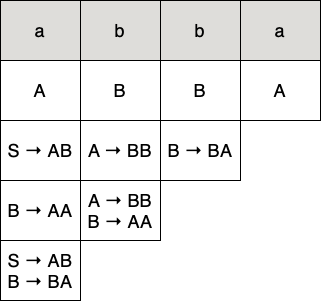
\includegraphics[scale=0.45]{CYK-Pyramide.png}
	\end{center}
	
	Der Ableitungsbaum lässt sich aus der Tabelle ablesen:
	
	\begin{center}
		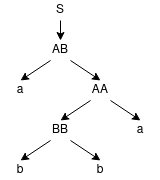
\includegraphics[scale=0.7]{Ableitungsbaum.png}
	\end{center}
		
\paragraph{(b)}
	\begin{enumerate}[label=\roman*.]
		\item
		Es gilt: $K\cdot R = \{k\circ r\ |\ \forall k \in K, r \in R\}$

		Die regulären Sprachen sind eine Teilmenge der kontextfreien Sprachen.
		Also ist auch $R$ kontextfrei. Kontextfreie Sprachen sind abgeschlossen unter \emph{Verkettung}: \\
		Sei $G_1 = (N_1, \Sigma_1, P_1, S_1)$ die kontextfreie Grammatik, welche $K$ erzeugt, und $G_2 = (N_2, \Sigma_2, P_2, S_2)$ die kontextfreie Grammatik, welche $R$ erzeugt. Dann kann eine kontextfreie Grammatik $G$ konstruiert werden, welche die Verkettung von $K$ und $R$ erzeugt:\\
		Man ergänze dafür ein neues Startsymbol $S$, sowie eine neue Produktionsregel $S \rightarrow S_1S_2$ und erhält $G = (N_1 \cup N_2 \cup \{S\}, \Sigma_1 \cup \Sigma_2, P_1 \cup P_2 \cup \{S \rightarrow S_1S_2\}, S)$.\\
		Da $L(G)=K\cdot R$ ist diese Sprache kontextfrei.

		Die Aussage ist also wahr.
				
		\item
		$L'$ ist bekanntermaßen nicht kontextfrei. Die Sprache $K = \{a^n\ |\ n \in \mathbb{N}_0\}$ über dem Alphabet $\Sigma = \{a,b,c\}$ ist regulär - denn es gilt $K = a^*$, also gibt es einen regulären Ausdruck für $K$ - und somit auch kontextfrei.\\
		Allerdings gilt auch für $K \circ L' = \{a^nb^mc^m\ |\ n,m \in \mathbb{N}_0\}$, das die Sprache regulär, mit Ausdruck: $K \circ L'= a^*(bc)^*$, und somit kontextfrei ist.
		
		Dieses Gegenbeispiel beweist, dass die Aussage falsch ist.
		
	\end{enumerate}
